\documentclass[11pt, a4paper]{article}
\usepackage[utf8]{inputenc}
\usepackage{amsmath,setspace,geometry}
\usepackage{amsthm}
\usepackage{amsfonts}
\usepackage[shortlabels]{enumitem}
\usepackage{rotating}
\usepackage{pdflscape}
\usepackage{graphicx}
\usepackage{bbm}
\usepackage[dvipsnames]{xcolor}
\usepackage{hyperref}
\hypersetup{colorlinks=true, linkcolor= BrickRed, citecolor = BrickRed, filecolor = BrickRed, urlcolor = BrickRed, hypertexnames = true}
\usepackage[]{natbib} 
\bibpunct[:]{(}{)}{,}{a}{}{,}
\geometry{left = 1.0in,right = 1.0in,top = 1.0in,bottom = 1.0in}
\usepackage[english]{babel}
\usepackage{float}
\usepackage{caption}
\usepackage{subcaption}
\usepackage{booktabs}
\usepackage{pdfpages}
\usepackage{threeparttable}
\usepackage{lscape}
\usepackage{bm}
\setstretch{1.4}
%\usepackage[tablesfirst,nolists]{endfloat}

\newtheorem{theorem}{Theorem}
\newtheorem{assumption}{Assumption}
\newtheorem{lemma}{Lemma}
\newtheorem{definition}{Definition}
\newtheorem{proposition}{Proposition}
\newtheorem{claim}{Claim}
\newtheorem{corollary}{Corollary}
\newtheorem{example}{Example}
\DeclareMathOperator{\rank}{rank}


\title{Finite Sample Performance of Conduct Parameter Test in Homogenous Good Markets}
\author{Yuri Matsumura\thanks{Department of Economics, Rice University. Email: Yuri.Matsumura@rice.edu} \and Suguru Otani \thanks{Department of Economics, Rice University. Email: so19@rice.edu
%Declarations of interest: none %this is for Economics Letters
}}

\begin{document}

\maketitle
\begin{abstract}
    We examine the finite sample performance of the conduct parameter test in homogeneous goods markets. The statistical power increases with (1) more markets, (2) a larger conduct parameter, and (3) a stronger demand rotation instrument. However, it remains challenging to reject the null hypothesis of perfect competition, even with a moderate number of markets (e.g., 1000) and five firms, regardless of the instrument's strength. We find that empirical findings failing to reject perfect competition are caused by the small number of markets, not by methodological flaws.
\vspace{0.1in}

\noindent\textbf{Keywords:} Conduct parameters, Homogenous goods market, Monte Carlo simulation, Statistical power analysis
\vspace{0in}
\newline
\noindent\textbf{JEL Codes:} C5, C13, L1

\bigskip
\end{abstract}


\section{Introduction}
Measuring competitiveness is an important task in the empirical industrial organization literature.
A conduct parameter is considered to be a useful measure of competitiveness. 
However, the parameter cannot be directly measured from data because data generally lack information about marginal costs.
Therefore, researchers endeavor to learn conduct parameters.

Researchers estimate and test structural models to understand firm conduct in both homogeneous and differentiated good markets \citep{nevoIdentificationOligopolySolution1998, magnolfi2022comparison, duarte2023testing}. 
We focus on homogenous good markets. 
The conduct parameters are identified for the linear model by \citet{bresnahan1982oligopoly}, and \cite{matsumura2023resolving} resolve conflicts between \cite{bresnahan1982oligopoly} and \cite{perloff2012collinearity} on identification problems. 
Estimation accuracy might improve by adding equilibrium existence conditions in the log-linear model \citep{matsumura2023mpec}. 
Conduct parameter testing is done by \cite{genesove1998testing}, who compare estimates from the sugar industry with direct measures of market power.\footnote{\cite{genesove1998testing} made mistakes on how to get predicted interaction terms of rotation demand instruments and endogenous quantity in the first stage regression. See Section A.3, \cite{matsumura2023resolving}.} 
When market power is around 0.1 and the number of markets is less than 100, perfect competition cannot be rejected. 
Also, \cite{steen1999testing} study 48 markets in the French salmon industry and \cite{shaffer1993test} study 25 markets in the Canadian banking industry. 
They cannot reject the null hypothesis that markets are perfectly competitive as well. 
Their results raise doubts about the methodology in itself \citep{shafferMarketPowerCompetition2017}.


While popular, there is a lack of formal Monte Carlo simulations for conduct parameter estimation and testing. 
To address this, we investigate the finite sample performance in homogeneous goods markets. 
We analyze statistical power by varying the number of markets, firms, and the strength of demand rotation instruments, under the null hypothesis of perfect competition.

Our findings reveal that statistical power increases with larger sample size (more markets), a larger conduct parameter, and stronger demand rotation instruments. 
Notably, even with a moderate number of markets (e.g., 1000) and five firms, we cannot achieve a rejection frequency of 80\% ($1-\beta=0.8$, where $\beta$ is the probability of a Type II error), regardless of instrument strength. 
This underscores the challenge of testing perfect competition, as noted by \cite{genesove1998testing}, \cite{steen1999testing}, and \cite{shaffer1993test}, because of the limited number of markets, rather than due to methodological flaws.

Our results and code provide a valuable reference for applied researchers examining assumptions about firm conduct in homogeneous goods markets, whether it's perfect competition, Cournot competition, or perfect collusion.

\section{Model}
Consider data with $M$ markets with homogeneous products.
Assume that there are $N$ firms in each market.
Let $m = 1,\ldots, M$ be the index for markets.
Then, we obtain a supply equation as follows:
\begin{align}
     P_m = -\theta\frac{\partial P_m(Q_{m})}{\partial Q_{m}}Q_{m} + MC_m(Q_{m}),\label{eq:supply_equation}
\end{align}
where $Q_{m}$ is the aggregate quantity, $P_m(Q_{m})$ is the demand function, $MC_{m}(Q_{m})$ is the marginal cost function, and $\theta\in[0,1]$ is  the conduct parameter. 
The equation nests perfect competition ($\theta=0$), Cournot competition ($\theta=1/N$), and perfect collusion ($\theta=1$). See \cite{bresnahan1982oligopoly}. 

Consider an econometric model that integrates the above model.
Assume that the demand and marginal cost functions are written as follows: 
\begin{align}
    P_m = f(Q_{m}, Y_m, \varepsilon^{d}_{m}, \alpha), \label{eq:demand}\\
    MC_m = g(Q_{m}, W_{m}, \varepsilon^{c}_{m}, \gamma),\label{eq:marginal_cost}
\end{align}
where $Y_m$ and $W_{m}$ are vectors of exogenous variables, $\varepsilon^{d}_{m}$ and $\varepsilon^{c}_{m}$ are error terms, and $\alpha$ and $\gamma$ are vectors of parameters.
Additionally, we have demand- and supply-side instruments, $Z^{d}_{m}$ and $Z^{c}_{m}$, and assume that the error terms satisfy the mean independence conditions, $E[\varepsilon^{d}_{m}\mid Y_m, Z^{d}_{m}] = E[\varepsilon^{c}_{m} \mid W_{m}, Z^{c}_{m}] =0$.

\subsection{Linear demand and cost}
Assume that linear demand and marginal cost functions are specified as follows:
\begin{align}
    P_m &= \alpha_0 - (\alpha_1 + \alpha_2Z^{R}_{m})Q_{m} + \alpha_3 Y_m + \varepsilon^{d}_{m},\label{eq:linear_demand}\\
    MC_m &= \gamma_0  + \gamma_1 Q_{m} + \gamma_2 W_{m} + \gamma_3 R_{m} + \varepsilon^{c}_{m},\label{eq:linear_marginal_cost}
\end{align}
where $W_{m}$ and $R_{m}$ are excluded cost shifters and $Z^{R}_{m}$ is Bresnahan's demand rotation instrument. 
The supply equation is written as follows:
\begin{align}
    P_m 
    %&= \gamma_0 + [\theta(\alpha_1 + \alpha_2Z^{R}_{m})+ \gamma_1] Q_{m}   + \gamma_2 W_{m} + \gamma_3 R_{m} + \varepsilon^{c}_{m}\nonumber\\ 
    &= \gamma_0 + \theta (\alpha_1 + \alpha_2 Z^{R}_m)Q_{m} + \gamma_1 Q_{m} + \gamma_2 W_m + \gamma_3 R_{m} +\varepsilon^c_m.\label{eq:linear_supply_equation}\end{align}
By substituting Equation \eqref{eq:linear_demand} with Equation \eqref{eq:linear_supply_equation} and solving it for $P_m$, we obtain the aggregate quantity $Q_{m}$ based on the parameters and exogenous variables as follows:
\begin{align}
    Q_{m} =  \frac{\alpha_0 + \alpha_3 Y_m - \gamma_0 - \gamma_2 W_{m} - \gamma_3 R_{m} + \varepsilon^{d}_{m} - \varepsilon^{c}_{m}}{(1 + \theta) (\alpha_1 + \alpha_2 Z^{R}_{m}) + \gamma_1}.\label{eq:quantity_linear}
\end{align}

\subsection{Optimal instruments}

To gain efficiency, we construct optimal instruments of \cite{chamberlain1987asymptotic}, which is used in demand estimation \citep{reynaert2014improving}.


\section{Simulation results}\label{sec:results}

\subsection{Simulation and estimation procedure}

We set true parameters and distributions as shown in Table \ref{tb:parameter_setting}. 
We vary the true value of $\theta$ from 0.05 (20-firms symmetric Cournot) to 1 (perfect collusion) and the strength of demand rotation instrument, $\alpha_2$, from 0.1 (weak) to 20.0 (extremely strong) which is unrealistically larger than the price coefficient level, $\alpha_1=1.0$.
For simulation, we generate 100 data sets.
We separately estimate the demand and supply equation by using two-stage least squares (2SLS) estimation.
The instrumental variables for demand estimation are $Z^{d}_{m} = (Z^{R}_{m}, Y_m, H_{m}, K_{m})$ and the instrumental variables for supply estimation are $Z^{c}_{m} = (Z^{R}_{m}, W_{m}, R_{m}, Y_m)$. 
The null hypothesis is that markets are under perfect competition, that is, $\theta=0$.
We compute the rejection
frequency as the power by using t-statistics at a significance level of 0.05 over 100 datasets.

\begin{table}[!htbp]
    \caption{True parameters and distributions}
    \label{tb:parameter_setting}
    \begin{center}
    \subfloat[Parameters]{
    \begin{tabular}{cr}
            \hline
            $\alpha_0$ & $10.0$  \\
            $\alpha_1$ & $1.0$  \\
            $\alpha_2$ & $\{0.1,0.5,1.0,5.0,20.0\}$ \\
            $\alpha_3$ & $1.0$  \\
            $\gamma_0$ & $1.0$ \\
            $\gamma_1$ & $1.0$  \\
            $\gamma_2$ & $1.0$ \\
            $\gamma_3$ & $1.0$\\
            $\theta$ & $\{0.05,0.1,0.2,0.33,0.5,1.0\}$ \\
            \hline
        \end{tabular}
    }
    \subfloat[Distributions]{
    \begin{tabular}{crr}
            \hline
            Demand shifter&  \\
            $Y_m$ & $N(0,1)$  \\
            Demand rotation instrument&   \\
            $Z^{R}_{m}$ & $N(10,1)$ \\
            Cost shifter&    \\
            $W_{m}$ & $N(3,1)$  \\
            $R_{m}$ & $N(0,1)$   \\
            $H_{m}$ & $W_{m}+N(0,1)$  \\
            $K_{m}$ & $R_{m}+N(0,1)$   \\
            Error&  &  \\
            $\varepsilon^{d}_{m}$ & $N(0,\sigma)$  \\
            $\varepsilon^{c}_{m}$ & $N(0,\sigma)$ \\
            \hline
        \end{tabular}
    }
    \end{center}
    \footnotesize
    Note: $\sigma=1.0$. $N:$ Normal distribution. $U:$ Uniform distribution.
\end{table}

Figure \ref{fg:theta_hat_power} presents the results of finite sample performance for the power of conduct parameter $\theta$.\footnote{See online appendix for simulation details and additional results of all other parameters.}
The rejection frequency increases when: (1) the sample size (number of markets) is large, (2) $\theta$ is large (number of firms is smaller), and (3) $\alpha_2$ is large (demand rotation instrument is stronger).
Panel (f) shows that with twenty firms ($\theta=0.05$) and a sufficiently large number of markets, we achieve approximately 70\% power to reject the null hypothesis of markets being under perfect competition.
However, we cannot reject the null hypothesis with acceptable sample size and power when markets are under twenty-firm symmetric Cournot competition.

A remarkable finding is that even with a moderate number of markets (e.g., 1000 in Panel (c)) and five firms, the rejection frequency cannot achieve 80\% (that is, $1-\beta=0.8$ where $\beta$ is the probability of making a Type II error), regardless of the strength of instruments.
This implies that \cite{genesove1998testing} using 97 markets, \cite{shaffer1993test} using 25 markets, and \cite{steen1999testing} using 48 markets, fail in rejecting perfect competition due to the small sample problem.


\begin{figure}[!ht]
  \begin{center}
  % \subfloat[M=50]{\includegraphics[width = 0.32\textwidth]
  % {figuretable/theta_hat_power_50.png}}
  \subfloat[$M=100$]{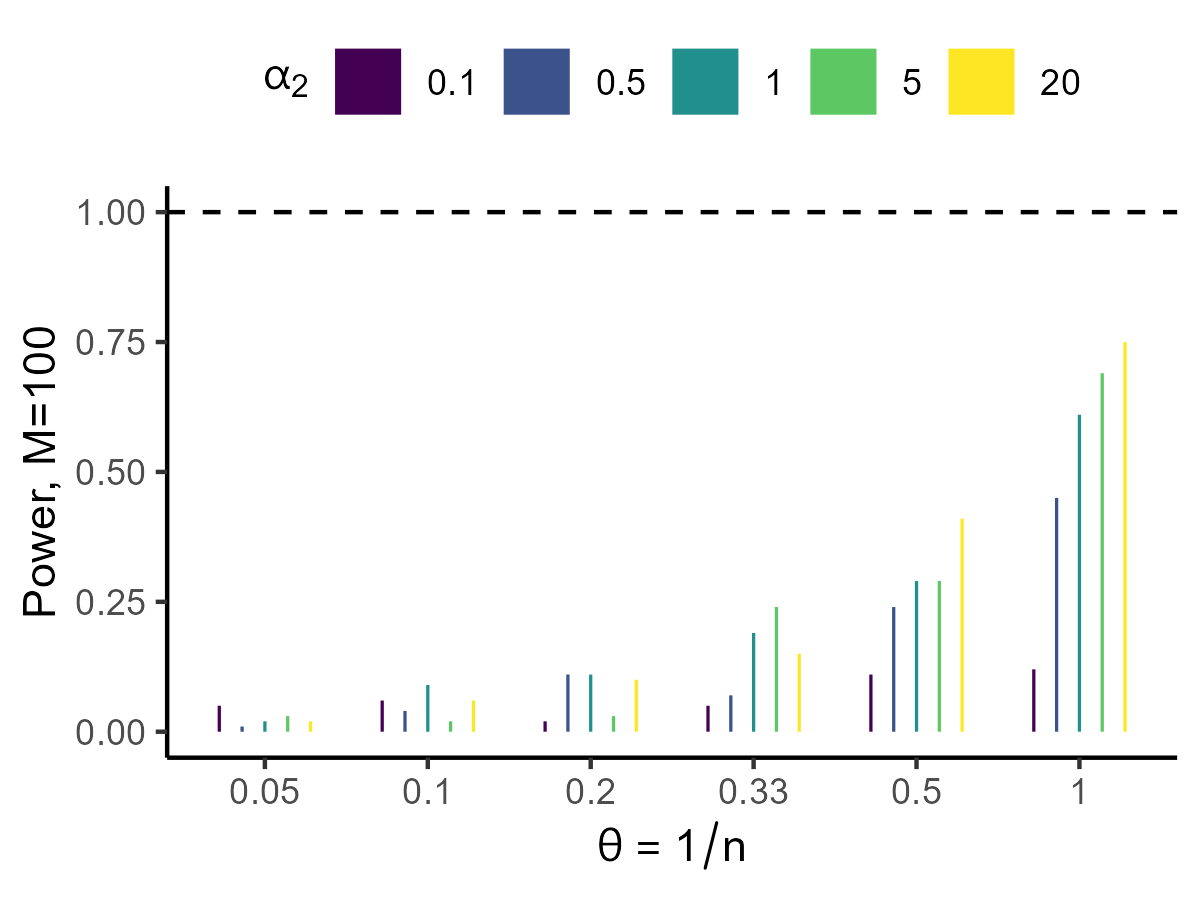
\includegraphics[width = 0.32\textwidth]
  {figuretable/theta_hat_power_100.png}}
  \subfloat[$M=200$]{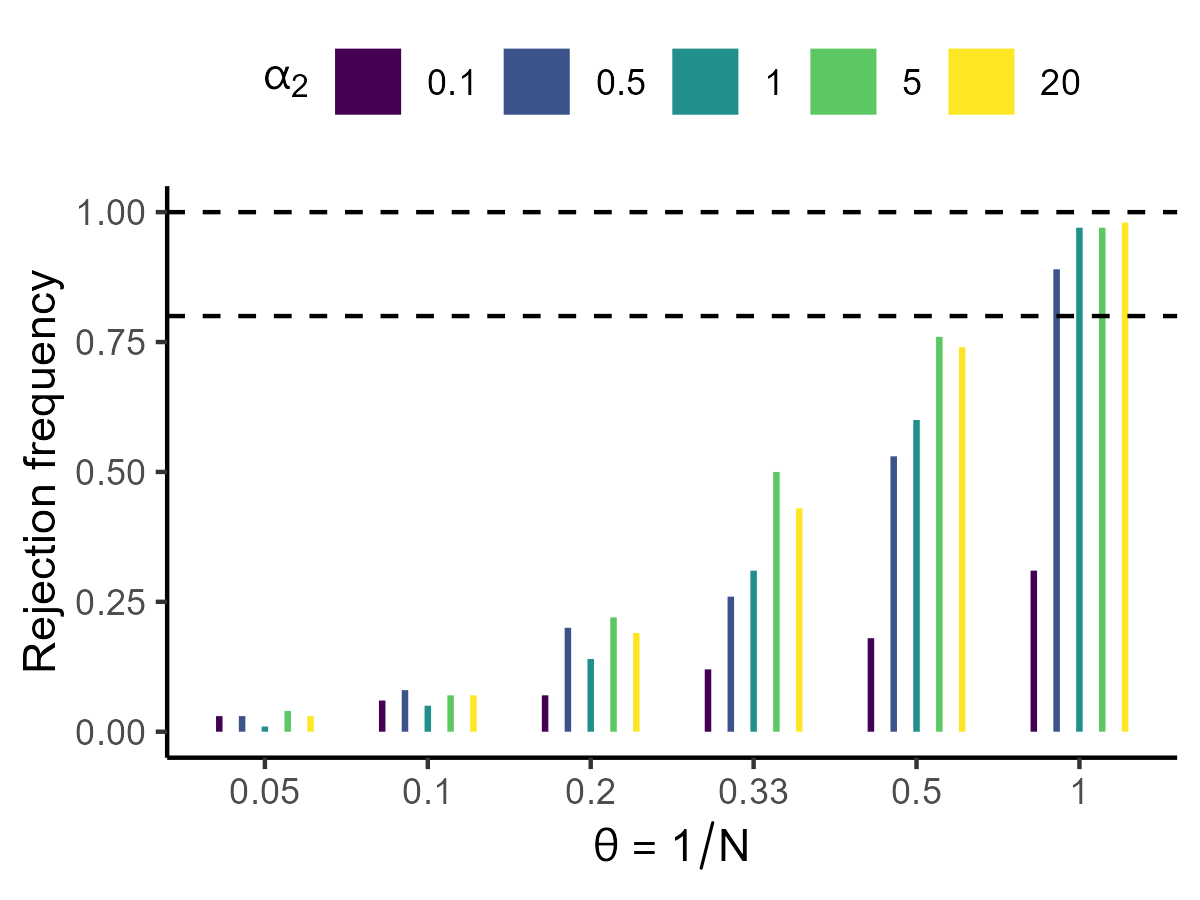
\includegraphics[width = 0.32\textwidth]
  {figuretable/theta_hat_power_200.png}}
  \subfloat[$M=1000$]{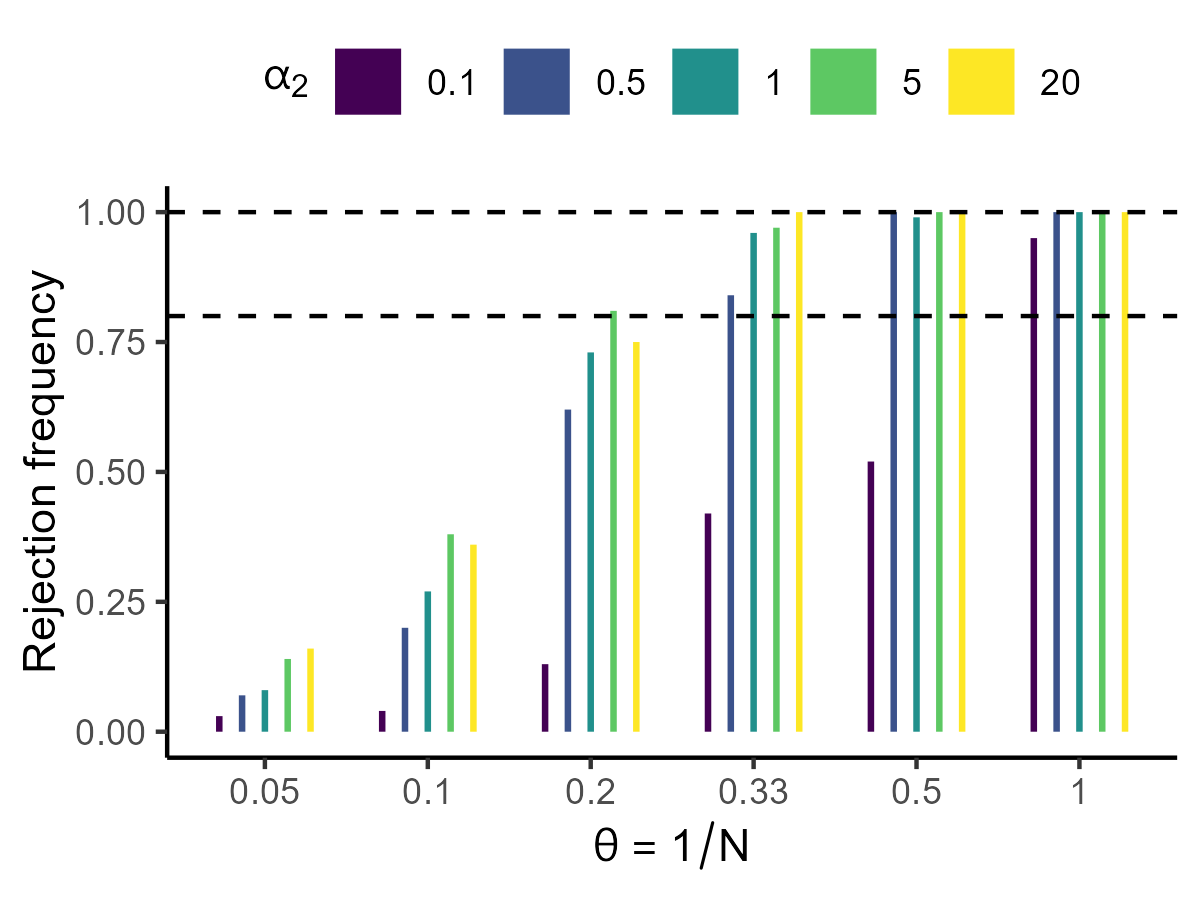
\includegraphics[width = 0.32\textwidth]
  {figuretable/theta_hat_power_1000.png}}\\
  \subfloat[$M=2000$]{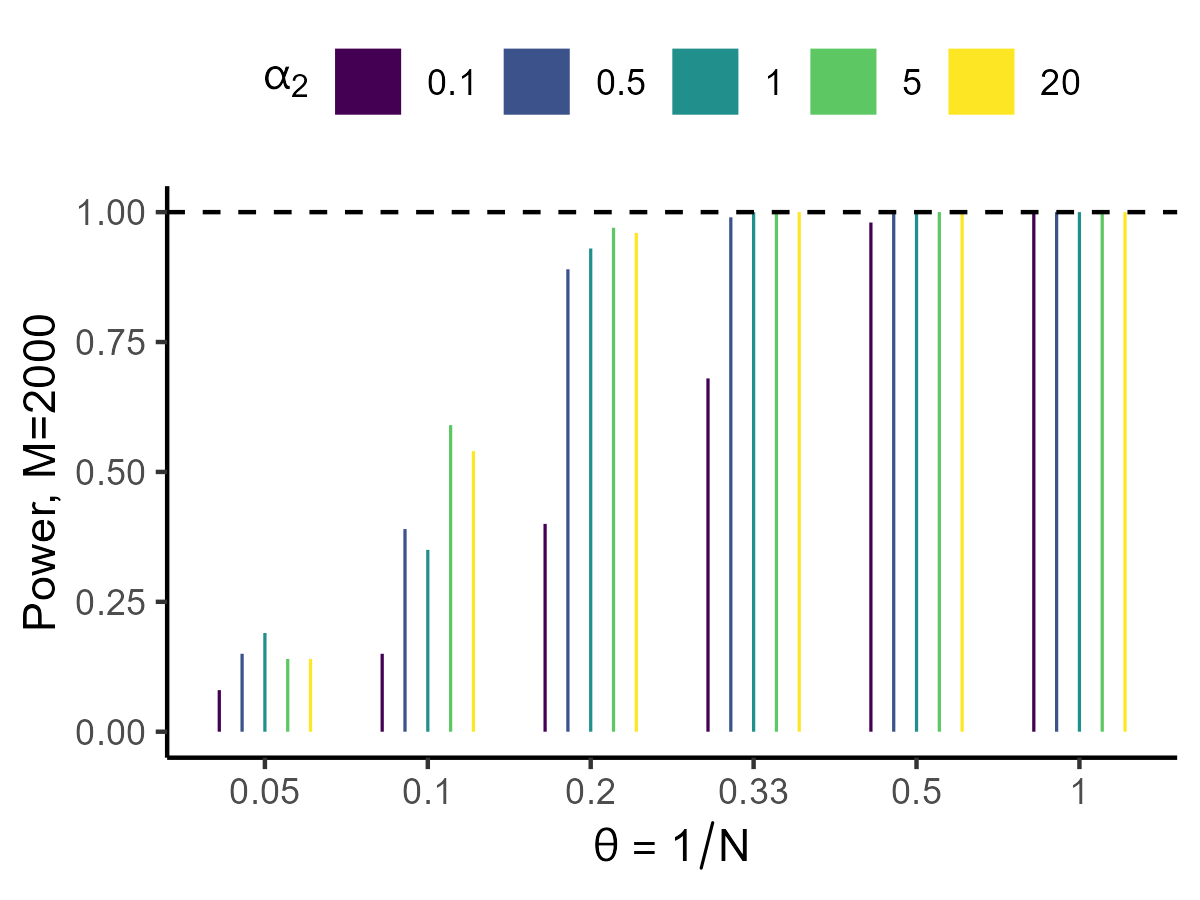
\includegraphics[width = 0.32\textwidth]
  {figuretable/theta_hat_power_2000.png}}
  \subfloat[$M=5000$]{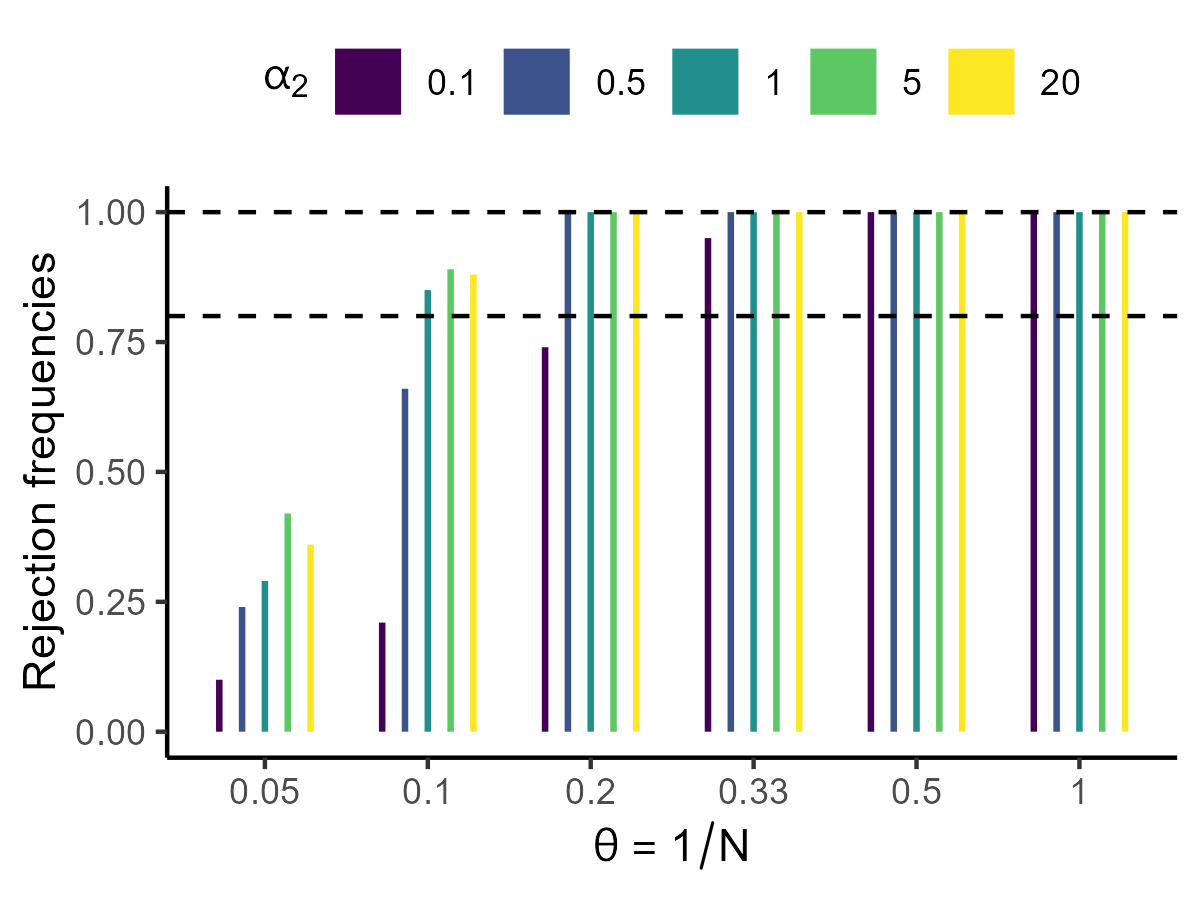
\includegraphics[width = 0.32\textwidth]
  {figuretable/theta_hat_power_5000.png}}
  \subfloat[$M=10000$]{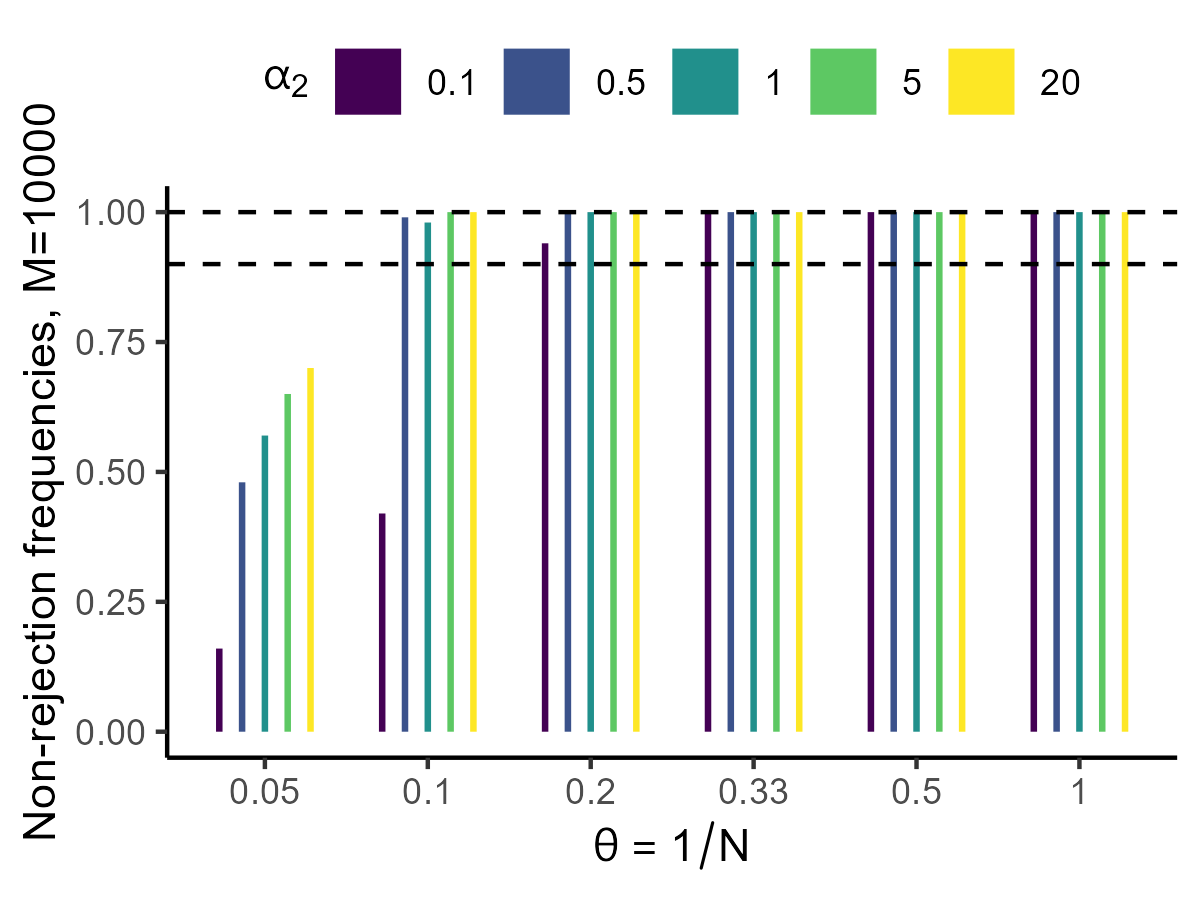
\includegraphics[width = 0.32\textwidth]
  {figuretable/theta_hat_power_10000.png}}
  \caption{Statistical power of conduct parameter $\theta$}
  \label{fg:theta_hat_power}
  \end{center}
  \footnotesize
  Note: Dotted lines are 80\% and 100\% rejection frequencies out of 100 simulation data.
\end{figure} 



\section{Conclusion}

We perform a statistical power analysis for conduct parameter estimation. 
The power increases with: (1) a large sample size (i.e., a large number of markets), (2) a large conduct parameter, and (3) a strong demand rotation instrument. 
However, rejecting the null hypothesis of markets being under perfect competition remains difficult, even with a moderate number of markets (e.g., 1000) and five firms, regardless of the instrument's strength. This confirms the challenge of testing perfect competition, as observed by \cite{genesove1998testing}, \cite{steen1999testing}, and \cite{shaffer1993test}, is caused by the small number of markets.


\paragraph{Acknowledgments}
We thank Jeremy Fox, Isabelle Perrigne, and Yuya Shimizu for their valuable advice. This research did not receive any specific grant from funding agencies in the public, commercial, or not-for-profit sectors. 

\newpage


\bibliographystyle{aer}
\bibliography{conduct_parameter}

\newpage

\setcounter{page}{1}
\appendix
\section{Online appendix}\label{sec:appendix}




\subsection{Details for our simulation settings}

To generate the simulation data, for each model, we first generate the exogenous variables $Y_m, Z^{R}_{m}, W_m, R_{m}, H_m$, and $K_m$ and the error terms $\varepsilon_{m}^c$ and $\varepsilon_{m}^d$ based on the data generation process in Table \ref{tb:parameter_setting}.
We compute the equilibrium quantity $Q_{m}$ for the linear model by \eqref{eq:quantity_linear}.
We then compute the equilibrium price $P_m$ by substituting $Q_{m}$ and other variables into the demand function \eqref{eq:linear_demand}.

We estimate the equations using the \texttt{ivreg} package in \texttt{R}.
An important feature of the model is that we have an interaction term of the endogenous variable $Q_{m}$ and the instrumental variable $Z^{R}_{m}$.
The \texttt{ivreg} package automatically detects that the endogenous variables are $Q_{m}$ and the interaction term $Z^{R}_{m}Q_{m}$, running the first stage regression for each endogenous variable with the same instruments. To confirm this, we manually write R code to implement the 2SLS model. 
When the first stage includes only the regression of $Q_{m}$, estimation results from our code differ from the results from \texttt{ivreg}. 
However, when we modify the code to regress $Z^{R}_{m}Q_{m}$ on the instrument variables and estimate the second stage by using the predicted values of $Q_{m}$ and $Z^{R}_{m}Q_{m}$, the result from our code and the result from \texttt{ivreg} coincide.

\subsection{Additional results}
Estimation results of all parameters except conduct parameter $\theta$ are shown on the author's github.

\subsection{Optimal instruments}
We define demand and supply residuals as follows.
\begin{align*}
    \varepsilon^{d}_{m}(\xi) &= P_m - \alpha_0 + (\alpha_1 + \alpha_2Z^{R}_{m})Q_{m} - \alpha_3 Y_m,\\
    \varepsilon^c_m(\xi) &= P_{m} - \gamma_0 - \theta (\alpha_1 + \alpha_2 Z^{R}_m)Q_{m} - \gamma_1 Q_{m} - \gamma_2 W_m - \gamma_3 R_{m}
\end{align*}
where $\xi=\left(\alpha_0, \alpha_1, \alpha_2, \alpha_3, \gamma_0, \gamma_1, \gamma_2, \gamma_3, \theta\right)$ is the $9\times 1$ parameter vector. 
Let $Z_{m}=(Z_{m}^{d},Z_{m}^{s})$ and $\varepsilon_{m}(\xi)=(\varepsilon_{m}^{d}(\xi),\varepsilon_{m}^{s}(\xi))'$.
We make the assumption that $\Omega=E[\varepsilon_{m}\varepsilon_{m}'|Z_{m}]$ is a constant $2\times 2$ matrix, defining the covariance structure of the demand and supply residuals.
 
The optimal instrument matrix of \cite{chamberlain1987asymptotic} is $g_{m}(Z_{m})=D_{m}(Z_{m})'\Omega^{-1}$
where the $2\times 9$ matrix $D_{m}(Z_{m})=E\left[\frac{\partial \varepsilon_{m}}{\partial \xi}| Z_{m}\right]$ is the conditional expectation of the derivative of the conditional moment restrictions with respect to parameters $\xi$. 

The conditional expectation $D_{m}(Z_{m})$ is difficult to compute, so most applications have considered approximations. As in \cite{reynaert2014improving}, we consider two types of approximation. 
The first approximation for $D_{m}(Z_{m})$ takes a second-order polynomial of $Z_{m}$ for the demand side instruments (first row of $D_{m}(Z_{m})$), i.e. cost shifters $W_{m}$ and $R_{m}$, and their squares and interactions, and $W_{m}$ and $R_{m}$ for the supply side instruments (second row of $D_{m}(Z_{m})$).
The second approximation for $D_{m}(Z_{m})$ implements the conditional expectation written as 
\begin{align*}
    &D_{m}(Z_{m})\\
    &=E\left[\frac{\partial \varepsilon_{m}}{\partial \xi}| Z_{m}\right]\\
    &=
    \begin{pmatrix}
    & E\left[\frac{\partial \varepsilon_{m}^{d}(\xi)}{\partial \alpha^{\prime}} \mid Z_{m}\right] & 
    E\left[\frac{\partial \varepsilon_{m}^{d}(\xi)}{\partial \gamma^{\prime}} \mid Z_{m}\right] & 
    E\left[\frac{\partial \varepsilon_{m}^{d}(\xi)}{\partial \theta} \mid Z_{m}\right]\\
    & E\left[\frac{\partial \varepsilon_{m}^{c}(\xi)}{\partial \alpha^{\prime}} \mid Z_{m}\right] & 
    E\left[\frac{\partial \varepsilon_{m}^{c}(\xi)}{\partial \gamma^{\prime}} \mid Z_{m}\right] & 
    E\left[\frac{\partial \varepsilon_{m}^{c}(\xi)}{\partial \theta} \mid Z_{m}\right]
    \end{pmatrix} \\
    &=\begin{pmatrix}
    -1 & 
    \overline{Q}_{m} & 
    Z^{R} \overline{Q}_{m} & 
    - Y_{m} &
    0 & 0 & 0 & 0 & 0 \\
    0 &- \theta \overline{Q}_{m} & -\theta Z^{R}_{m}\overline{Q}_{m} & 0 & 
    -1 &
    - \overline{Q}_{m} &
    -W_{m} &
    -R_{m} &
    -(\alpha_1 + \alpha_2 Z^{R}_{t})\overline{Q}_{m}
    \end{pmatrix}
\end{align*}
where $ \overline{Q}_{m} \equiv E[Q_{m}\mid Z_{m}]$.
In our model, $E[Q_{m}\mid Z_{m}]$ can be explicitly obtained because $E[\varepsilon_{t}^{d}\mid Z_{t}^{R}] = E[\varepsilon_{t}^{c}\mid Z_{t}^{R}] = 0 $:
\begin{align*}
    E[Q_{m}\mid Z_{m}] &=E\left[\left.\frac{\alpha_0 + \alpha_3 Y_m - \gamma_0 - \gamma_2 W_{m} - \gamma_3 R_{m} + \varepsilon^{d}_{m} - \varepsilon^{c}_{m}}{(1 + \theta) (\alpha_1 + \alpha_2 Z^{R}_{m}) + \gamma_1}\right| Z_{m}\right] \\
    & = \frac{\alpha_0 + \alpha_3 Y_m - \gamma_0 - \gamma_2 W_{m} - \gamma_3 R_{m}}{(1 + \theta) (\alpha_1 + \alpha_2 Z^{R}_{m}) + \gamma_1},\\
    E[Z^{R}_{m}Q_{m}\mid Z_{m}] &=E\left[\left. Z^{R}_{m}\frac{\alpha_0 + \alpha_3 Y_m - \gamma_0 - \gamma_2 W_{m} - \gamma_3 R_{m} + \varepsilon^{d}_{m} - \varepsilon^{c}_{m}}{(1 + \theta) (\alpha_1 + \alpha_2 Z^{R}_{m}) + \gamma_1}\right | Z_{m}\right]\\
    & = Z^{R}_{m}\frac{\alpha_0 + \alpha_3 Y_m - \gamma_0 - \gamma_2 W_{m} - \gamma_3 R_{m}}{(1 + \theta) (\alpha_1 + \alpha_2 Z^{R}_{m}) + \gamma_1},\\
    E[(\alpha_1 + \alpha_2 Z^{R}_m)Q_{m}\mid Z_{m}] &=E\left[\left. (\alpha_1 + \alpha_2 Z^{R}_m)\frac{\alpha_0 + \alpha_3 Y_m - \gamma_0 - \gamma_2 W_{m} - \gamma_3 R_{m}}{(1 + \theta) (\alpha_1 + \alpha_2 Z^{R}_{m}) + \gamma_1}\right | Z_{m}\right]\\
    &= (\alpha_1 + \alpha_2 Z^{R}_m)\frac{\alpha_0 + \alpha_3 Y_m - \gamma_0 - \gamma_2 W_{m} - \gamma_3 R_{m}}{(1 + \theta) (\alpha_1 + \alpha_2 Z^{R}_{m}) + \gamma_1}.
\end{align*}

When only the supply side is estimated, the earlier optimal instrument matrix is modified into $g_{m}(Z_{m})=D_{m}(Z_{m})'$ where 
\begin{align*}
    D_{m}(Z_{m}) &= \begin{pmatrix}
    & E\left[\frac{\partial \varepsilon_{m}^{c}(\xi)}{\partial \alpha^{\prime}} \mid Z_{m}\right] & 
    E\left[\frac{\partial \varepsilon_{m}^{c}(\xi)}{\partial \gamma^{\prime}} \mid Z_{m}\right] & 
    E\left[\frac{\partial \varepsilon_{m}^{c}(\xi)}{\partial \theta} \mid Z_{m}\right]
    \end{pmatrix} \\
    &=\begin{pmatrix}
    0 &- \theta \overline{Q}_{m} & -\theta Z^{R}_{m}\overline{Q}_{m} & 0 & 
    -1 &
    \overline{Q}_{m} &
    -W_{m} &
    -R_{m} &
    -(\alpha_1 + \alpha_2 Z^{R}_m)\overline{Q}_{m}
    \end{pmatrix}
\end{align*}

\end{document}